\documentclass[11pt]{article}
\usepackage[a4paper,margin=2.3cm]{geometry}
\usepackage{amsmath,amssymb,amsthm}
\usepackage{graphicx}
\usepackage{booktabs}
\usepackage[hidelinks]{hyperref}
\usepackage{xcolor}
\usepackage{caption}
\usepackage{titlesec}
\usepackage{tikz}
\usepackage{enumitem}
\titleformat{\section}{\large\bfseries}{\thesection}{0.7em}{}
\newcommand{\fig}[1]{figures/#1}
\newcommand{\Z}{\mathbb Z}

\theoremstyle{plain}
\newtheorem{theorem}{Theorem}
\newtheorem{proposition}[theorem]{Proposition}
\newtheorem{corollary}[theorem]{Corollary}
\newtheorem{lemma}[theorem]{Lemma}
\theoremstyle{definition}
\newtheorem{definition}[theorem]{Definition}
\theoremstyle{remark}
\newtheorem{remark}[theorem]{Remark}

\title{\bfseries Machine-checked fragments of a\\ base-10 prime pattern}
\author{Elizabeth Johnson (\texttt{@Ellyrox110}) \and Jeromie Beasley (ORCID \href{https://orcid.org/0009-0006-4645-5643}{0009-0006-4645-5643})}
\date{Working report, revision 7}

\begin{document}
\maketitle

\begin{abstract}
\noindent
This report records the results obtained on top of a pre-existing framework, and keeps the two
apart. The framework (the base-10 encoding of primes, the end-digit key, the twin segmentation and
the colour scheme) is Elizabeth Johnson's and was published earlier. The results here are new and
joint. The main ones are an exact count, $3^{n+1}-2^{n+1}$, of the \emph{admissible} residue words
of length $n$, together with a proof that every word produced by consecutive twin primes is one of
them, so that the count is an upper bound for the realised words; a proof that only the prime $5$
ever obstructs; the equilibrium obstruction; the exact range of the coprimality test; and a
description of the base-10 colour wheel in coordinates, $\Z/10\cong\Z/2\times\Z/5$, on which every
twin pair above $5$ avoids the neutral hue. Some supporting facts (digit exclusivity for twin
pairs, the uniqueness of $3,5,7$, the carry identity) are classical or elementary and are included
because the formalisation needs them. The census, admissibility at $5$ of every realised word, the
equilibrium obstruction and the wheel identities at $W=10$ are formalised in Lean~4 with Mathlib,
and every axiom footprint is reported.
\end{abstract}

\section*{Authorship}

\begin{center}
\begin{tabular}{@{}p{0.46\textwidth}p{0.46\textwidth}@{}}
\toprule
\textbf{Elizabeth Johnson (prior work)} & \textbf{Jointly (this report)}\\
\midrule
$p=10s+d$ encoding; inner nodes & the census $A(n)=3^{n+1}-2^{n+1}$; realised $\Rightarrow$ admissible\\
end-digit key $g\equiv d_2-d_1 \pmod{10}$ & the carry identity (elementary)\\
mod-9 twin classes & the obstruction table (mod 2, 3, 5)\\
twin segmentation; counterflow framing & the seven word classes\\
the colour scheme (attribution under verification; see note) & digit exclusivity; junction uniqueness (classical; proofs included)\\
rung ladder $D=(g\bmod 10)/2+1$ & the equilibrium obstruction; the range of the coprimality test\\
 & the wheel in coordinates; twins on the wheel\\
 & the Lean formalisations\\
\bottomrule
\end{tabular}
\end{center}

\noindent
\textbf{Citation.} For the framework alone, cite her manuscript
\emph{EJ's Alternate Base Prime Number Pattern and the Twin Prime Counterflow Model},
DOI \href{https://doi.org/10.5281/zenodo.23378596}{10.5281/zenodo.23378596}.
For anything in this report, cite both authors and that manuscript.

\smallskip
\noindent\textbf{Posting.} Posted by Jeromie Beasley with Elizabeth Johnson's knowledge; she may fork it or request changes (2026-11-04). The split above cites her framework to her alone and the new results to both.

\smallskip
\noindent\textbf{Attribution note.} A related document, \emph{Advanced Color Theory in Relations to
Primes} (Elizabeth Johnson and Shaun Neer, October 2026), lists a second author. The attribution of
the colour scheme and its mixing rules, credited here to Elizabeth Johnson, is still being verified
with the authors, and will be corrected in a later revision if needed.

\section{Notation and the framework}

\paragraph{Primes and digits.} Every prime $p>5$ is written $p=10s+d$, with \emph{end digit}
$d\in\{1,3,7,9\}$ and \emph{inner node} $s$.

\paragraph{Twin starts and gaps.} A \emph{twin start} is a prime $a$ with $a+2$ also prime. We list
them in increasing order:
\[
a_1=3,\quad a_2=5,\quad a_3=11,\quad a_4=17,\quad a_5=29,\ \dots
\]
and write $d_k=a_{k+1}-a_k$ for the gaps (always with an index, to distinguish them from end
digits), so that $d_1=2$ and $d_2=d_3=6$. Every twin start
$a\ge5$ satisfies $a\equiv5\pmod 6$, because $a$ and $a+2$ are both coprime to $6$. Hence
\begin{equation}\label{eq:mod6}
d_k\equiv 0 \pmod 6\qquad (k\ge 2).
\end{equation}
We call $a_k$ \emph{regular} if $a_k\ge 11$, that is, $k\ge3$. The first two twin starts, $3$ and
$5$, are the \emph{seed}: they share the prime $5$.

\paragraph{Segments.} A \emph{segment} runs from $bg=a_k$ (a twin start) to $ep=a_{k+1}+2$ (the end
of the \emph{next} twin). The primes strictly between $bg$ and $ep$ are its \emph{interior primes}.
The \emph{twin-to-twin gap} is $\gamma_k=a_{k+1}-(a_k+2)$.

\begin{theorem}[two channels]\label{thm:two}
For integers $p<q$ with $p=10s_p+d_p$, $q=10s_q+d_q$ and $0\le d_p,d_q\le 9$,
\[
q-p=10\,\Delta s+\Delta d,\qquad \Delta s=s_q-s_p,\quad \Delta d=d_q-d_p .
\]
Consequently
\[
\Delta s=\Big\lfloor \frac{q-p}{10}\Big\rfloor+\mathbb 1[\Delta d<0].
\]
\end{theorem}
\begin{proof}
The first identity is substitution. For the second: $-9\le\Delta d\le 9$, so
$q-p=10\Delta s+\Delta d$ gives floor $=\Delta s$ when $\Delta d\ge 0$ and $\Delta s-1$ when
$\Delta d<0$.
\end{proof}

\noindent
This is a substitution identity. The gap splits into a bounded digit channel and an unbounded node
channel. Among
consecutive primes above $5$ in the first $5\cdot10^6$, the carry $\mathbb 1[\Delta d<0]$ fires on
$39.73\%$ of gaps.

\section{The residue language of the twin gaps}

\subsection{Words and admissibility}

By \eqref{eq:mod6} a regular gap is $\equiv0\pmod 6$, so its last digit $r=d\bmod10$ lies in
$\{0,2,4,6,8\}$ and determines $d\bmod 30$:
\begin{center}
\begin{tabular}{@{}c|ccccc@{}}
$r$ & 0 & 2 & 4 & 6 & 8\\\hline
$d \bmod 30$ & 0 & 12 & 24 & 6 & 18
\end{tabular}
\end{center}

\begin{definition}\label{def:word}
A \emph{word} of length $n$ is $w=(r_1,\dots,r_n)\in\{0,2,4,6,8\}^n$. Let $\delta_i$ be the
residue mod $30$ assigned to $r_i$ by the table, put $D_0=0$ and $D_i=\delta_1+\dots+\delta_i$, and
define the \emph{offset set}
\[
\Delta(w)=\bigcup_{i=0}^{n}\{D_i,\;D_i+2\}\subseteq \Z/30 .
\]
The word is \emph{admissible} if, for each $q\in\{2,3,5\}$, the reduction of $\Delta(w)$ mod $q$ is
not all of $\Z/q$. The word \emph{realised from} $a_k$ is $(d_k\bmod10,\dots,d_{k+n-1}\bmod10)$.
\end{definition}

If $w$ is realised from $a_k$, the $2n+2$ numbers $a_k+D'_i$ and $a_k+D'_i+2$, where the $D'_i$
are the true partial sums $d_k+\dots+d_{k+i-1}$, are the twin primes $a_{k+i}$ and $a_{k+i}+2$. Their
offsets from $a_k$ reduce to $\Delta(w)$ modulo $2$, $3$ and $5$.

\begin{theorem}[realised words are admissible]\label{thm:realised}
Every word realised from a regular twin start is admissible.
\end{theorem}
\begin{proof}
Let $q\in\{2,3,5\}$. If $\Delta(w)$ covered $\Z/q$, then some member $a_k+D'_i$ or $a_k+D'_i+2$
of the tuple would be $\equiv0\pmod q$. That member is prime, so it equals $q\le5$. But every
member is at least $a_k\ge11$, which is a contradiction.
\end{proof}

\begin{remark}[the seed is a genuine exception]\label{rem:seed}
The hypothesis $a_k\ge 11$ cannot be dropped. From $a_2=5$ the twin starts $5,11,17$ realise the
word $(6,6)$, with offsets $\{0,2,6,8,12,14\}\equiv\{0,1,2,3,4\}\pmod 5$. This word is not
admissible, and the proof fails because the tuple contains the prime $5$ itself. If windows were
allowed to start at $5$, the counts of realised words below would read $5,20,66,212,666$ instead of
$5,19,65,211,665$.
\end{remark}

\begin{theorem}[only $5$ obstructs]\label{thm:obstruct}
For every word, $\Delta(w)\bmod 2=\{0\}$ and $\Delta(w)\bmod 3=\{0,2\}$. Hence a word is admissible
if and only if $\Delta(w)\bmod 5\ne\Z/5$.
\end{theorem}
\begin{proof}
Every $\delta_i\equiv0\pmod 6$, so every $D_i\equiv0$ modulo $2$ and $3$. The set
$\bigcup_i\{D_i,D_i+2\}$ therefore reduces to $\{0\}$ mod $2$ and to $\{0,2\}$ mod $3$, and neither
covers its modulus.
\end{proof}

\subsection{The census}

\begin{theorem}[census]\label{thm:census}
The number of admissible words of length $n$ is
\[
A(n)=3^{\,n+1}-2^{\,n+1}.
\]
\end{theorem}
\begin{proof}
\emph{Step 1: walk positions.} Write $r_i=2\ell_i$ with $\ell_i\in\{0,1,2,3,4\}$; this $\ell_i$ is
the rung index, one less than the rung of the framework's ladder. Since $\delta_i\equiv r_i\pmod{10}$,
we have $\delta_i\equiv2\ell_i\pmod5$, so $D_i\equiv 2c_i\pmod 5$ with
\[
c_0=0,\qquad c_i=\ell_1+\dots+\ell_i \pmod 5 .
\]
The map $(\ell_1,\dots,\ell_n)\mapsto(c_1,\dots,c_n)$ is a bijection $(\Z/5)^n\to(\Z/5)^n$, with
inverse $\ell_i=c_i-c_{i-1}$.

\emph{Step 2: reduce to positions.} Let $V=\{c_0,\dots,c_n\}$ be the set of visited positions. Then
$\Delta(w)\bmod5=2\cdot\bigl(V\cup(V+1)\bigr)$, and multiplication by $2$ is a bijection of $\Z/5$.
By Theorem~\ref{thm:obstruct}, $w$ is admissible iff $V\cup(V+1)\ne\Z/5$.

\emph{Step 3: the cover lemma.} $V\cup(V+1)$ misses a point $m$ iff $m\notin V$ and $m-1\notin V$,
that is, iff $V\subseteq\{m+1,m+2,m+3\}$. So $w$ is admissible iff $V$ lies in a consecutive
triple. Since $0=c_0\in V$, the triple contains $0$, and there are exactly three such triples:
\[
t_0=\{0,1,2\},\qquad t_1=\{4,0,1\},\qquad t_2=\{3,4,0\}.
\]

\emph{Step 4: inclusion--exclusion.} By Steps 1--3, $A(n)$ is the number of
$(c_1,\dots,c_n)\in(\Z/5)^n$ with all $c_i$ in one of $t_0,t_1,t_2$. Each box $t_j^{\,n}$ has $3^n$
elements. The pairwise intersections are $\{0,1\}^n$, $\{0,4\}^n$ and $\{0\}^n$, of sizes $2^n$,
$2^n$ and $1$, and the triple intersection is $\{0\}^n$. Hence
\[
A(n)=3\cdot 3^n-\bigl(2^n+2^n+1\bigr)+1=3^{\,n+1}-2^{\,n+1}.\qedhere
\]
\end{proof}

\begin{remark}[the converse is not claimed]
The converse of Theorem~\ref{thm:realised}, that every admissible word is realised from some
regular twin start, is a statement of prime-tuples type and is \textbf{not} proved here. It has
been checked computationally that for $n\le5$ the words realised from regular twin starts within
the first $5\cdot10^6$ primes are exactly the admissible ones. Nothing beyond that range is claimed.
\end{remark}

\begin{center}
\includegraphics[width=\textwidth]{\fig{fig1_census.pdf}}
\captionof{figure}{Left: the count $3^{n+1}-2^{n+1}$ against the number of words realised from
regular twin starts in the first $5\cdot10^6$ primes ($5,19,65,211,665$). Right: the admissible
share $A(n)/5^n=3(3/5)^n-2(2/5)^n$ decays like $(3/5)^n$, so almost all long residue words are
impossible.}
\end{center}

\begin{center}
\includegraphics[width=0.75\textwidth]{\fig{fig5_obstruction.pdf}}
\captionof{figure}{Maximum number of distinct residues reached, per modulus, over all words up to
length $8$. Only mod $5$ can reach its modulus.}
\end{center}

\subsection{The seven word classes}

Call $b_i=2c_i\bmod 10\in\{0,2,4,6,8\}$ the \emph{beam} at step $i$. By Step~1 of the proof above,
and because every $D_i$ is even, $b_i\equiv D_i\pmod{10}$. In beam coordinates the three triples are
$T_0=\{0,2,4\}$, $T_1=\{0,2,8\}$ and $T_2=\{0,6,8\}$ (from $t_0,t_1,t_2$). We sort the
admissible words by exactly which of these contain all their beams. The counts below follow from
the same inclusion--exclusion and were also confirmed by enumeration for $n\le6$.

\begin{center}
\begin{tabular}{@{}llrrrrrr@{}}
\toprule
class & beams & closed form & $n=1$ & 2 & 3 & 4 & 5\\
\midrule
$T_0$ only & $\subseteq\{0,2,4\}$ & $3^n-2^n$ & 1 & 5 & 19 & 65 & 211\\
$T_1$ only & $\subseteq\{0,2,8\}$ & $3^n-2^{n+1}+1$ & 0 & 2 & 12 & 50 & 180\\
$T_2$ only & $\subseteq\{0,6,8\}$ & $3^n-2^n$ & 1 & 5 & 19 & 65 & 211\\
$T_0T_1$ only & $\subseteq\{0,2\}$, not all $0$ & $2^n-1$ & 1 & 3 & 7 & 15 & 31\\
$T_1T_2$ only & $\subseteq\{0,8\}$, not all $0$ & $2^n-1$ & 1 & 3 & 7 & 15 & 31\\
$T_0T_2$ only & --- & $0$ & 0 & 0 & 0 & 0 & 0\\
$T_0T_1T_2$ & all beams $0$ & $1$ & 1 & 1 & 1 & 1 & 1\\
\midrule
total & & $3^{n+1}-2^{n+1}$ & 5 & 19 & 65 & 211 & 665\\
\bottomrule
\end{tabular}
\end{center}

\noindent
Three consequences follow.
\begin{itemize}[nosep]
\item $T_0$ and $T_2$ have equal counts. This is because $t_0$ and $t_2$ each meet one neighbouring
triple in two points and the other in one point, while $t_1$ meets both neighbours in two points.
\item The beams $4$ and $6$ never occur in the same admissible word, since no triple containing $0$
contains both $2$ and $3$. This is a statement about beams (positions). It is \emph{not} a statement
about letters: the word $(4,6)$, with beams $4,0$, is admissible, and the adjacent letters $4,6$ or
$6,4$ occur $30\,124$ times in the data.
\item Class ``$T_0T_2$ only'' is empty: $t_0\cap t_2=\{0\}$, and the all-zero word also lies in $T_1$.
\end{itemize}

\begin{center}
\includegraphics[width=0.7\textwidth]{\fig{fig2_classes.pdf}}
\captionof{figure}{The seven classes at $n=5$, summing to $665$. The figure labels the classes
$T_0,T_1,T_2$ as A, B, C.}
\end{center}

\section{Digits, junctions and equilibrium}

\begin{theorem}[digit exclusivity]\label{thm:digit}
Let $(a,a+2)$ be a twin pair with $a>5$. Then $a$ ends in $1$, $7$ or $9$, and $a+2$ ends in $3$,
$9$ or $1$. In particular, a twin start ending in $3$ is $3$ itself, and a twin end ending in $7$ is
$7$ itself.
\end{theorem}
\begin{proof}
Since $a>5$ is prime, $a$ is odd and $5\nmid a$. If $a\equiv3\pmod{5}$ then $5\mid a+2$ with
$a+2>5$, which is impossible. So $a\bmod 5\in\{1,2,4\}$, and since $a$ is odd, $a\bmod10\in\{1,7,9\}$.
Then $a+2\bmod10\in\{3,9,1\}$. For the last sentence: $3$ and $7$ are not among the allowed digits for
$a>5$, and the cases $a\le5$ are $(3,5)$ and $(5,7)$.
\end{proof}
\begin{remark}
Primes ending in $3$ above $3$, and primes ending in $7$ above $7$, both exist ($13,23,43$ and
$17,37,47$). The theorem is about the two positions in a \emph{twin pair}, not about all primes. The statement is classical; it is included because the formalisation uses it.
\end{remark}


\begin{theorem}[junction uniqueness]\label{thm:junction}
Among $p-2,p,p+2$ exactly one is divisible by $3$. Consequently, if all three are prime then $p=5$,
and the twin-to-twin gap $\gamma_k$ vanishes only for $k=1$.
\end{theorem}
\begin{proof}
The three numbers are pairwise distinct mod $3$ because $2\not\equiv0\pmod 3$, so exactly one is
$\equiv0$. If all three are prime, that one equals $3$, so $p\in\{1,3,5\}$; only $p=5$ makes all
three prime. Finally, $\gamma_k=0$ means $a_k+2=a_{k+1}$, so $a_k,a_k+2,a_k+4$ are all prime, and
then $a_k=3$.
\end{proof}

\begin{theorem}[equilibrium obstruction]\label{thm:eq}
Say equilibrium holds at $k$ if $d_k=d_{k+1}$, i.e.\ $a_k,a_{k+1},a_{k+2}$ are in arithmetic
progression. Let $a_k$ be regular, and let $u=a_k\bmod10$ and $v=a_{k+1}\bmod10$ (both in
$\{1,7,9\}$ by Theorem~\ref{thm:digit}). If equilibrium holds at $k$, then
\[
a_{k+2}\equiv 2v-u\pmod{10}\quad\text{and}\quad 2v-u\bmod 10\in\{1,7,9\}.
\]
Of the nine cells $u\to v$, exactly four violate this: $1\to7$, $7\to1$, $9\to1$ and $9\to7$. In
those cells equilibrium is impossible.
\end{theorem}
\begin{proof}
$a_{k+2}=a_{k+1}+d_{k+1}=a_{k+1}+d_k=2a_{k+1}-a_k$, so $a_{k+2}\equiv2v-u\pmod{10}$. Since
$a_{k+2}>a_k\ge11$ is a twin start, its last digit lies in $\{1,7,9\}$ by Theorem~\ref{thm:digit}.
The table lists the nine cells.
\end{proof}

\begin{center}
\begin{tabular}{@{}ccccl@{}}
\toprule
cell $u\to v$ & $r=v-u \bmod 10$ & $2v-u\bmod10$ & equilibrium & \\
\midrule
$1\to1$, $7\to7$, $9\to9$ & 0 & $1,7,9$ & possible & \\
$7\to9$ & 2 & 1 & possible & \\
$9\to1$ & 2 & 3 & impossible & \\
$7\to1$ & 4 & 5 & impossible & \\
$1\to7$ & 6 & 3 & impossible & \\
$1\to9$ & 8 & 7 & possible & \\
$9\to7$ & 8 & 5 & impossible & \\
\bottomrule
\end{tabular}
\end{center}

\noindent
In terms of the gap residue $r=d_k\bmod10$: the residues $4$ and $6$ never equilibrate; the residues
$2$ and $8$ equilibrate only from the single cells $7\to9$ and $1\to9$ respectively; and the residue
$0$ can equilibrate from all three of its cells. Over regular twin starts in the first $5\cdot10^6$
primes, the four impossible cells show exactly zero equilibria, and the five possible cells show
equilibrium rates between $1.66\%$ and $2.48\%$. The spread among the possible cells is studied
empirically in \texttt{03-docs/THEOREMS.md}; it is not a theorem of this report.

\noindent\emph{Notation note.} The framework documents label a cell by $bg\to ep$, the end digit of
$a_k$ and of $a_{k+1}+2$, i.e.\ $u\to v+2$. In that notation the impossible cells are
$1\to9$, $7\to3$, $9\to3$ and $9\to9$.

\section{The range of the coprimality test}

\begin{theorem}\label{thm:range}
Let $P$ be a product of distinct primes, and let $p$ be the smallest prime not dividing $P$. Let
$n>1$ be an integer.
\begin{enumerate}[nosep]
\item[(a)] If $\gcd(n,P)>1$ and $n$ is not itself a prime factor of $P$, then $n$ is composite;
\item[(b)] if $\gcd(n,P)=1$ and $n<p^2$, then $n$ is prime;
\end{enumerate}
and $n=p^2$ is the smallest $n>1$ with $\gcd(n,P)=1$ that is composite.
\end{theorem}
\begin{proof}
(a) A prime factor $q$ of $P$ divides $n$, and $n\ne q$. (b) Every prime below $p$ divides $P$, so
every prime factor of $n$ is at least $p$. A composite $n$ would therefore satisfy $n\ge p^2$.
Finally, $p^2$ is coprime to $P$ and composite, and by (b) nothing smaller is.
\end{proof}

\noindent
The end digit tests coprimality to $10$: $n\bmod10\in\{1,3,7,9\}$ iff $\gcd(n,10)=1$. On its own
($P=10$, $p=3$) it confirms primality only below $9$. Adding the test $3\nmid n$ gives the
$30$-wheel ($P=30$, $p=7$), which confirms primality exactly up to $n<49$; $49=7^2$ is the first
failure. Every such finite test therefore refutes reliably but confirms only below $p^2$. Deciding
larger $n$ requires enlarging $P$ as $n$ grows, which is trial division.

\section{The colour wheel}

The colour scheme of the framework labels the ten digits: primaries $1,3,7,9$, secondaries
$2,4,6,8$, grey $5$, base $0$. This section shows how much of that labelling is intrinsic to the ring $\Z/10$
and how much is convention. The orbit partition, the two layers, the hue coordinate and complement
as negation are forced. The direction of the hue circle, and which orbit is called primary, are
choices. It then places the twin primes on the resulting wheel.
The words \emph{layer}, \emph{hue} and \emph{grey} below are names for coordinates. No colorimetric
or physical claim is made (Remark~\ref{rem:not}).

\subsection{Orbits}

\begin{theorem}[orbits]\label{thm:wheel}
Let $W\ge2$. The orbits of the unit group $(\Z/W)^\times$ acting on $\Z/W$ by multiplication are
the classes $\{x:\gcd(x,W)=g\}$, one for each divisor $g\mid W$. The class with $W/g=m$ has
$\varphi(m)$ elements. At $W=10$ the four orbits are
\[
\{0\},\qquad \{5\},\qquad \{2,4,6,8\},\qquad \{1,3,7,9\}.
\]
\end{theorem}
\begin{proof}
Multiplying by a unit does not change $\gcd(x,W)$. Conversely, suppose $\gcd(x,W)=\gcd(y,W)=g$, and
put $m=W/g$, $x=gx'$, $y=gy'$ with $x',y'$ units mod $m$. Choose $t$ with $tx'\equiv y'\pmod m$. Let
$W'$ be the largest divisor of $W$ coprime to $m$. By the Chinese remainder theorem there is $u$
with $u\equiv t\pmod m$ and $u\equiv1\pmod{W'}$. Every prime factor of $W$ divides $m$ or $W'$, so
$u$ is a unit mod $W$. Then $ux-y=g(ux'-y')$ and $m\mid ux'-y'$, so $W\mid ux-y$. For the size: the
orbit of $x$ consists of the residues $g\,x''$ with $x''$ a unit mod $m$, and $g\,x''$ determines
$x''\bmod m$. So the orbit has $\varphi(m)$ elements.
\end{proof}

\begin{proposition}\label{prop:2p}
The orbit sizes are $1,1,m,m$ for some $m$ if and only if $W=2p$ with $p$ an odd prime, in which
case $m=p-1$. This gives the family $W=6,10,14,22,26,34,38,\dots$
\end{proposition}
\begin{proof}
Orbits correspond to divisors, so $W$ has exactly four divisors: $W=q^3$ or $W=qr$ with primes
$q<r$. For $W=q^3$ the sizes are $1,q-1,q(q-1),q^2(q-1)$; two of them equal $1$ only if $q=2$, which
gives $1,1,2,4$, not of the required shape. For $W=qr$ the sizes are $1,q-1,r-1,(q-1)(r-1)$; two
ones force $q=2$, and then the sizes are $1,1,r-1,r-1$. Conversely, $W=2p$ gives these sizes.
\end{proof}

\subsection{The wheel in coordinates}

\begin{theorem}[coordinates]\label{thm:coords}
Let $W=2p$ with $p$ an odd prime. Write $\lambda(x)=x\bmod2$ (the \emph{layer}) and $h(x)=x\bmod p$
(the \emph{hue}). Then $x\mapsto(\lambda(x),h(x))$ is a ring isomorphism $\Z/2p\to\Z/2\times\Z/p$,
and the following hold.
\begin{enumerate}[nosep]
\item[(a)] The four orbits are $\{(0,0)\}$, $\{(1,0)\}$ (the \emph{grey} point $p$),
$\{(0,h):h\ne0\}$ and $\{(1,h):h\ne0\}$.
\item[(b)] A unit $u$ acts by $(\lambda,h)\mapsto(\lambda,\bar u\,h)$ with $\bar u=u\bmod p$, and
$u\mapsto\bar u$ is an isomorphism $(\Z/2p)^\times\to(\Z/p)^\times$, a cyclic group of order $p-1$.
Fix a generator $\gamma$ of $(\Z/p)^\times$ and define the \emph{angle} of a non-grey hue by
$h=\gamma^{\theta}$, $\theta\in\Z/(p-1)$. Then every unit acts on the non-neutral points of each layer as a
rotation $\theta\mapsto\theta+j$, simply transitively. The non-neutral points of each layer
therefore form a circle of $p-1$ hues.
\item[(c)] Complementation $x\mapsto-x$ is the half turn $\theta\mapsto\theta+\tfrac{p-1}2$, and it
preserves layers.
\item[(d)] Adding the grey point, $x\mapsto x+p$, swaps the two layers and keeps the hue.
\end{enumerate}
\end{theorem}
\begin{proof}
The map is the Chinese remainder isomorphism. (a) This is Theorem~\ref{thm:wheel} in coordinates.
For instance, $\gcd(x,2p)=1$ iff $\lambda=1$ and $h\ne0$. (b) A unit is odd, so it fixes $\lambda$.
The reduction map is a bijection because a unit is determined by its residue mod $p$, its layer
being $1$. Cyclicity holds because $p$ is prime. (c) $-1=\gamma^{(p-1)/2}$ in $(\Z/p)^\times$.
(d) $p$ corresponds to $(1,0)$.
\end{proof}

\begin{remark}[what depends on the generator]\label{rem:gen}
The angle $\theta$ depends on the choice of $\gamma$. Replacing $\gamma$ by $\gamma^{j}$, with $j$
a unit mod $p-1$, multiplies every angle by $j^{-1}$. Up to rotation and reflection this gives
$\varphi(p-1)/2$ different cyclic orders of the hues. That is one order for $p=5$ and $7$, where
only the orientation is a choice, and two for $p=11$ and $13$, which we checked by enumeration. The
partition into orbits, the layers, the hue coordinate and the half turn $x\mapsto-x$ do not depend
on any choice.
\end{remark}

\noindent
At $W=10$ take $\gamma=2$; it is realised by the unit $7$, since $7\equiv2\pmod5$. Multiplication by
$7$ is the quarter turn:
\begin{center}
\begin{tabular}{@{}lcccc@{}}
\toprule
angle $\theta$ & 0 & 1 & 2 & 3\\
hue $h=2^\theta \bmod 5$ & 1 & 2 & 4 & 3\\
\midrule
odd layer (primaries) & 1 & 7 & 9 & 3\\
even layer (secondaries) & 6 & 2 & 4 & 8\\
\bottomrule
\end{tabular}
\qquad
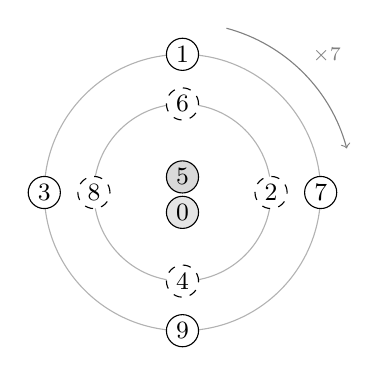
\begin{tikzpicture}[baseline=(c.base),scale=0.9]
\node (c) at (0,0) {};
\draw[gray!60] (0,0) circle (1.95);
\draw[gray!60] (0,0) circle (1.25);
\foreach \a/\o/\e in {90/1/6, 0/7/2, 270/9/4, 180/3/8} {
  \node[circle,draw,fill=white,inner sep=1.5pt,font=\small] at (\a:1.95) {$\o$};
  \node[circle,draw,dashed,fill=white,inner sep=1.5pt,font=\small] at (\a:1.25) {$\e$};
}
\node[circle,draw,fill=gray!30,inner sep=1.5pt,font=\small] at (0,0.22) {$5$};
\node[circle,draw,fill=black!10,inner sep=1.5pt,font=\small] at (0,-0.28) {$0$};
\draw[->,gray] (75:2.4) arc (75:15:2.4) node[midway,above right,font=\scriptsize] {$\times7$};
\end{tikzpicture}
\end{center}

\noindent
So at $W=10$ the scheme of the framework is recovered from the ring structure, up to the
orientation of the circle and the choice of which orbit to call primary. There is a neutral axis
$\{0,5\}$. Each layer has four non-neutral points arranged as a circle of hues, with the framework's
primaries on the unit layer. Each
primary $x$ has a secondary partner $x+5$ of the same hue: $1\!-\!6$, $7\!-\!2$, $9\!-\!4$,
$3\!-\!8$. The complementary pairs $\{1,9\},\{7,3\},\{6,4\},\{2,8\}$ are exactly the opposite points
of each circle, and complementary digits add to the base: $x+(-x)=0$.

\subsection{Twin primes on the wheel}

\begin{proposition}[twins avoid grey]\label{prop:twinhue}
Let $(a,a+2)$ be a twin pair with $a>5$. Both members lie on the unit layer and have non-grey hue.
More precisely, $h(a)\in\{1,2,4\}$ (angles $0,1,2$; digits $1,7,9$) and $h(a+2)=h(a)+2\in\{3,4,1\}$
(angles $3,2,0$; digits $3,9,1$). The same argument at any odd prime $q<a$ gives
$a\bmod q\notin\{0,\,q-2\}$.
\end{proposition}
\begin{proof}
Both members are primes greater than $5$, hence odd and coprime to $5$. $h(a)\ne0$, and
$h(a+2)=h(a)+2\ne0$ forces $h(a)\ne3$. The general statement is the same argument mod $q$.
\end{proof}

\noindent
This is Theorem~\ref{thm:digit} in wheel coordinates, and it connects the two halves of the report.
The twin step $x\mapsto x+2$ \emph{translates} the hue additively. Theorem~\ref{thm:coords} shows
that the wheel symmetries are \emph{multiplications}, which rotate hue. Twin structure therefore
lives in the additive structure of the ring and the wheel symmetry in the multiplicative one. The
census has the same reading. Every member of a realised tuple has a non-grey hue. Admissibility at
$5$ says that the offset pattern $\bar\Delta(w)=\Delta(w)\bmod5$ can be translated off the grey hue:
there is an $h_0\in\Z/5$ with $0\notin h_0+\bar\Delta(w)$. This is immediate: take $h_0=-m$ for any
$m\notin\bar\Delta(w)$. Theorem~\ref{thm:census} thus counts the \emph{words} whose hue pattern can
be translated off grey. Different words can share a pattern.

\begin{remark}[what the wheel does not do]\label{rem:not}
The orbits classify a \emph{label system} on $\Z/W$. Nothing here is a claim about perceived or
physical colour, and the words layer, hue and grey are names for coordinates. On prime gaps: a unit
$u$ permutes the residues coprime to $W$, so it fixes the set of wheel survivors. We checked by
enumeration at $W=10,30,210,2310$ that only $u=1$ preserves the cyclic order of the survivors and
only $u=-1$ reverses it. For instance, the $30$-wheel gap cycle $6,4,2,4,2,4,6,2$ is a palindrome
up to rotation. The unit multiplications therefore contribute exactly the reflection symmetry of the
wheel's gap pattern. They act on residues only, not on the primes themselves.
\end{remark}

\subsection{Colour at scale}\label{sec:scale}

``Scale'' has two meanings here, and the arithmetic treats them differently. \emph{Resolution} means
reading more digits: colouring $n$ by $n\bmod 10^k$ instead of $n\bmod 10$. \emph{Magnitude} means
looking at larger numbers. The first is exact. The second is statistical.

\paragraph{Resolution: the tower of wheels.} Reduction mod $10^k$ is a ring map
$\pi:\Z/10^{k+1}\to\Z/10^{k}$, the \emph{projection} from one scale to the next coarser one. By
Theorem~\ref{thm:wheel} the colour classes of the $10^k$-wheel are the gcd classes
$g=2^i5^j$, $0\le i,j\le k$, so there are $(k+1)^2$ of them.

\begin{proposition}[classes refine]\label{prop:refine}
Projection sends each class of $\Z/10^{k+1}$ into a single class of $\Z/10^{k}$, namely the one with
$\gcd$ equal to $\gcd(g,10^k)$. Over the four classes of the $10$-wheel, the $10^k$-wheel has
\[
\underbrace{1}_{\text{primaries}}\;+\;\underbrace{k}_{\text{secondaries}}\;+\;
\underbrace{k}_{\text{grey}}\;+\;\underbrace{k^2}_{\text{base}}\;=\;(k+1)^2
\]
classes, the \emph{shades} of each colour. In particular the primaries never split: $n$ is a unit
mod $10^k$ iff it is a unit mod $10$. Every prime above $5$ lies in this single class at every scale.
\end{proposition}
\begin{proof}
$\gcd(x\bmod 10^k,10^k)=\gcd(x,10^k)=\gcd(\gcd(x,10^{k+1}),10^k)$. Iterating down to scale $10$:
a class $2^i5^j$ lies over the primaries iff $i=j=0$; over the secondaries iff $i\ge1$, $j=0$ ($k$
choices); over grey iff $i=0$, $j\ge1$ ($k$ choices); and over the base iff $i,j\ge1$ ($k^2$
choices).
\end{proof}

\noindent
At scale $100$, for example, the secondaries split into two shades (divisible by $2$ only, and by
$4$). Grey splits into two (divisible by $5$ only, and by $25$, i.e.\ $25$ and $75$). The base
splits into four. The hue of the unit class is the coordinate $n\bmod 5^k$. Its circle is the
cyclic group $(\Z/5^k)^\times$, which has $N_k=4\cdot5^{k-1}$ elements: $4$ hues at scale $10$, $20$
at scale $100$, $100$ at scale $1000$.

\begin{definition}\label{def:circle}
A \emph{hue circle} at scale $10^k$ is the cyclic order $x,gx,g^2x,\dots$ on $(\Z/5^k)^\times$
given by a generator $g$; it does not depend on the starting point $x$. The circle of $h$ at scale
$10^{k+1}$ \emph{refines} the circle of $g$ at scale $10^k$ if $h\equiv g\pmod{5^k}$, equivalently
if projection sends each step $y\mapsto hy$ to the step $\pi(y)\mapsto g\,\pi(y)$.
\end{definition}

\begin{proposition}[zooming keeps the coarse order]\label{prop:zoom}
Let $g$ generate $(\Z/5^{k})^\times$. Then $g\bmod5$ generates $(\Z/5)^\times$, so $g\equiv2$ or
$3\pmod 5$. Projected to scale $10$, the circle of $g$ is the coarse circle of $2$, traversed
$5^{k-1}$ times: forwards if $g\equiv2$, backwards if $g\equiv3$. In particular a circle that
refines the coarse circle of $2$, in the sense of Definition~\ref{def:circle} iterated, runs
forwards.
\end{proposition}
\begin{proof}
Reduction $(\Z/5^k)^\times\to(\Z/5)^\times$ is a surjective homomorphism (every unit mod $5$ lifts),
so it sends a generator to a generator. The generators mod $5$ are $2$ and $3=2^{-1}$. If
$g\equiv2^{\pm1}\pmod5$, then from any start $x$ the coarse hue of the $\theta$-th step is
$\bar x\,2^{\pm\theta}$. That expression advances the coarse angle by $\pm1$ at every step, and the
$N_k=4\cdot5^{k-1}$ steps of the fine circle make $5^{k-1}$ coarse turns.
\end{proof}

\begin{proposition}[how much freedom each zoom adds]\label{prop:freedom}
\leavevmode
\begin{enumerate}[nosep]
\item[(a)] At scale $10^k$ there are $\varphi(N_k)$ hue circles, or $\varphi(N_k)/2$ up to reflection:
$1$, $4$, $20$ for $k=1,2,3$.
\item[(b)] A given circle at scale $10$ has exactly $4$ refinements at scale $100$. Every circle at
scale $10^k$ with $k\ge2$ has exactly $5$ refinements at scale $10^{k+1}$.
\item[(c)] The circles of $2$ refine one another at every scale: $2$ generates $(\Z/5^k)^\times$
for every $k$.
\end{enumerate}
\end{proposition}
\begin{proof}
(a) The circle of $g$ determines $g$ as the successor of $1$, and reading the circle backwards gives
the circle of $g^{-1}\ne g$ (as $N_k>2$). So there is one circle per generator.
(b) The refinements of the circle of $g$ are the generators mod $5^{k+1}$ among the five lifts
$g+j5^k$. A unit mod $p^{k+1}$, with $p$ an odd prime and $k\ge 2$, is a generator iff its
reduction mod $p^2$ is \cite{IR}. All five lifts have the same reduction mod $25$ as $g$, so all
five are generators. For $k=1$: the solutions of $x^4\equiv1\pmod{25}$ form a subgroup of order
$4$ with exactly one element over each unit mod $5$ ($1,7,18,24$ over $1,2,3,4$). A lift of a
generator mod $5$ has order $4$ or $20$, and it has order $4$ exactly when it is that element. So
exactly $4$ of the $5$ lifts generate. For $g=2$ the exception is $7$.
(c) $2$ has order $20$ mod $25$, and a primitive root mod $p^2$ is a primitive root mod every $p^k$
\cite{IR}.
\end{proof}

\noindent
At scale $100$ the four refinements of the coarse circle of $2$ start, after $1$, with
$2,4,8,16$, or $12,19,3,11$, or $17,14,13,21$, or $22,9,23,6$. Each reads the coarse hues
$1,2,4,3$ five times round. So zooming in preserves the coarse cyclic order exactly once an
orientation is fixed, and it still leaves real freedom in the fine order: a finite set of
refinements at each step (4 at the first zoom, then 5 at every later zoom). The circle of $2$ is a
canonical choice that is coherent at every scale.

Two cautions. First, the unit class carries more than its hue: $(\Z/100)^\times\cong C_2\times
C_{20}$, where the extra $C_2$ is $n\bmod4$. That layer coordinate $n\bmod2^k$ refines into
$(\Z/2^k)^\times$, which is \emph{not} cyclic for $k\ge3$ ($(\Z/8)^\times\cong C_2\times C_2$). So
from scale $1000$ on, the layer side does not form a single circle. Second, hue circles are defined
here for the unit class only. How to give hue to the other shades is open.

\paragraph{Magnitude: the colour proportions drift.} By the prime number theorem for arithmetic progressions,
each of the four primaries ends exactly $1/4$ of the primes asymptotically. At any finite size
the proportions are not equal, and the following are \emph{measurements} over the first
$5\cdot10^6$ primes above $5$, not theorems.
\begin{itemize}[nosep]
\item \emph{A persistent lead.} The primes ending in $3$ or $7$ (the non-squares mod $10$) were
never strictly behind those ending in $1$ or $9$ (the squares), checked at every prime. They were
tied only at $p=11,31,41,3581$. This is Chebyshev's bias. Under the generalised Riemann hypothesis
and a linear-independence hypothesis, Rubinstein and Sarnak \cite{RS} showed that such a lead holds
on a set of logarithmic density strictly between $0$ and $1$. So it is expected to fail eventually,
on a small but positive proportion of the logarithmic scale: it is persistent, not permanent.
\item \emph{An order that churns.} Ranking the four digits by count at $60$ logarithmically spaced
checkpoints gives $49$ checkpoints with no tie, and the ranking changes $36$ times between
consecutive ones. Seven different rankings occur. Checked at every prime, $3$ is strictly last in
four stretches, starting at $p=3571$, $55\,619$, $55\,639$ and $56\,311$.
\item \emph{A fading repulsion.} The share of consecutive primes with the same last digit was
$11.84\%$ below $10^4$, $15.35\%$ below $10^6$ and $17.12\%$ over all $5\cdot10^6$ primes, against
$25\%$ for independent digits. Lemke Oliver and Soundararajan \cite{LOS} found this bias and gave a
conjectural explanation through the Hardy--Littlewood conjectures, in which it decays very slowly,
roughly like $1/\log x$. It lives exactly in the sixteen end-digit cells of the framework, which is
why no cell count in this work is treated as a constant.
\end{itemize}
These figures are computed by \texttt{04-verification/scale\_check.py}.

\noindent
\emph{Summary.} Under zooming, the coarse cyclic order is preserved exactly, once an orientation is
chosen, and each zoom adds a finite, explicitly counted freedom in the fine order
(Propositions~\ref{prop:zoom}--\ref{prop:freedom}). Under growth there is a persistent but not
permanent bias, with the finer ranking churning beneath it. The theory of that bias is conditional
(Rubinstein--Sarnak) or conjectural (Lemke Oliver--Soundararajan). Both kinds of scale show a coarse
structure that persists while the finer order moves, but only the first is a theorem.

\subsection{What a theory built on this seed has, and what it still needs}

\emph{Established here.} The wheel $\Z/2\times\Z/p$ has a neutral axis and two layers, each with a
circle of $p-1$ hues on which the units act by rotation, and complement is the half turn. The
partition and coordinates are forced by the ring, and the cyclic order of the hues is forced up to
the choices in Remark~\ref{rem:gen}. The primes above $p$ occupy the unit layer. Twin pairs above
$q$ avoid hue $0$ and hue $-2$ at every odd prime $q$. The census counts the words whose hue pattern
can be translated off grey. Across scales, the wheels form a tower in which classes refine and the
primaries never split. Each zoom preserves the oriented coarse hue order and adds a finite, counted
freedom in the fine order (Section~\ref{sec:scale}).

\emph{Open, and stated as open.}
\begin{itemize}[nosep]
\item[(i)] \emph{A mixing law.} The ring supplies two candidate operations: addition, which adds hues
and layers, and multiplication, which rotates hues. Which of them, if either, should model
``mixing'' is a modelling decision, not a theorem. Under addition, complements mix to the base, as
noted above.
\item[(ii)] \emph{Finer wheels.} Proposition~\ref{prop:2p} gives one wheel for each odd prime. Every
admissible word can be lifted to gap sequences that are admissible at every prime: by the Chinese
remainder theorem, choose the gaps $\equiv0$ modulo all primes $\ge7$ up to any bound. What is open
is the converse of Theorem~\ref{thm:realised}, which needs two things. One is a prime $k$-tuples
statement, that such tuples actually occur. The other is consecutiveness: no further twin pair may
fall between the members. The Hardy--Littlewood conjecture alone does not give the second.
\item[(iii)] \emph{Rates.} Whether the measured equilibrium rates (Section~3) can be expressed
through hue statistics is untested.
\item[(iv)] \emph{Choosing the order at every scale.} Proposition~\ref{prop:freedom} says what the
choices are. Whether the framework wants the canonical circle of $2$, or some other coherent family,
is a modelling decision. So is how to treat the non-cyclic layer side from scale $1000$ on.
\item[(v)] \emph{Shades.} Proposition~\ref{prop:refine} gives the shades of each colour at every
scale. Whether shades should carry their own order (for instance by the exponents $i,j$) is open.
\item[(vi)] \emph{Delays beyond 5.} The free-hue weights $\omega_q$ at every prime, and the
correction for consecutiveness (Section~\ref{sec:delay}), are the natural next quantitative target.
\end{itemize}

\section{Delays on the wheel}\label{sec:delay}

A \emph{delay} is the waiting time until something recurs. This section treats two kinds. The
first is the delay, counted in primes, until an end digit comes back. The second is the delay,
measured in integers, between twin pairs. The rule for the second is exact; how well it describes
the primes is measured, and every measurement below is computed by
\texttt{04-verification/delay\_check.py} on the first $5\cdot10^6$ primes above $5$.

\subsection{Return delays of a colour}

For a sequence in which a colour has frequency $f$, the mean delay between its occurrences is
$1/f$ up to boundary terms. This is because the delays sum to the distance from the first
occurrence to the last. Each primary has frequency $1/4$ asymptotically (Section~\ref{sec:scale}),
so its mean return delay is $4$. The data give $4.001$, $3.999$, $4.000$, $4.000$ for the digits
$1,3,7,9$. The \emph{rate fixes the mean, but not the shape}:

\begin{center}
\begin{tabular}{@{}lrrrrr@{}}
\toprule
delay (primes) & 1 & 2 & 3 & 4 & 5\\
\midrule
digit $3$ & $16.59\%$ & $21.42\%$ & $17.19\%$ & $12.63\%$ & $9.16\%$\\
digit $1$ & $17.65\%$ & $20.00\%$ & $17.22\%$ & $12.76\%$ & $9.26\%$\\
independent digits & $25.00\%$ & $18.75\%$ & $14.06\%$ & $10.55\%$ & $7.91\%$\\
\bottomrule
\end{tabular}
\end{center}

\noindent
An immediate return is strongly suppressed, and delays $2$ to $5$ are correspondingly enhanced.
This is the bias of Lemke Oliver and Soundararajan \cite{LOS} seen as a waiting time. Its range is
short. The mutual information between a digit and the digit $k$ primes later is $36.5$, $2.0$ and
$0.11$ millibits for $k=1,2,3$ (out of an entropy of $2$ bits per digit), and below $0.15$
millibits for $k\ge3$. So the memory of the colour sequence lasts about two primes.

\subsection{Twin delays are weighted by free hues}

\begin{proposition}[free hues]\label{prop:free}
Let $h$ be the delay between two twin pairs $(a,a+2)$ and $(a+h,a+h+2)$. The number of hues
$a\bmod5$ for which all four members avoid the grey hue $0$ is
\[
\omega_5(h)=5-\bigl|\{0,2,h,h+2\}\bmod 5\bigr| \;=\; 3,\ 1,\ 2,\ 2,\ 1
\qquad\text{for } h\equiv0,1,2,3,4\pmod5 .
\]
More generally, at any prime $q\ge3$ the count is $\omega_q(h)=q-|\{0,2,h,h+2\}\bmod q|$.
\end{proposition}
\begin{proof}
A hue $a$ fails exactly when $a\equiv-u$ for some $u$ in the offset pattern $\{0,2,h,h+2\}$, and
distinct offsets give distinct failing hues. List the five patterns mod $5$ to get the values.
\end{proof}

\noindent
$\omega_5(h)$ is exactly the number of translations of the offset pattern off grey
(Section~\ref{sec:scale}, and the census reading after Proposition~\ref{prop:twinhue}). It is also
the local factor at $5$ of the Hardy--Littlewood conjecture for the tuple $\{0,2,h,h+2\}$. That
conjecture predicts that the number of twin pairs at distance $h$ (not necessarily consecutive)
grows in proportion to the singular series
$\mathfrak S(h)=\prod_q\bigl(1-\nu_q(h)/q\bigr)(1-1/q)^{-4}$, where $\nu_q(h)=q-\omega_q(h)$ is the
number of residues the pattern occupies. The factor at $q=5$ is proportional to $\omega_5(h)$.
For delays between twin starts above $5$, $h\equiv0\pmod 6$, so the factors at $2$ and $3$ do not
depend on $h$. Averaging the factors at $q\ge7$ over $h$ in each class mod $5$, it predicts shares proportional to $3:1:2:2:1$, i.e.\ $33.3\%$, $11.1\%$, $22.2\%$,
$22.2\%$, $11.1\%$. This is a prediction of a conjecture, not a theorem. Measured:

\begin{center}
\begin{tabular}{@{}lrrrrr@{}}
\toprule
delay $h \bmod 5$ & 0 & 1 & 2 & 3 & 4\\
free hues $\omega_5(h)$ & 3 & 1 & 2 & 2 & 1\\
\midrule
predicted share & $33.3\%$ & $11.1\%$ & $22.2\%$ & $22.2\%$ & $11.1\%$\\
all pairs of twin starts, $h\le3000$ & $33.1\%$ & $11.1\%$ & $22.3\%$ & $22.2\%$ & $11.2\%$\\
consecutive twin pairs & $30.7\%$ & $12.1\%$ & $24.1\%$ & $22.1\%$ & $11.1\%$\\
\bottomrule
\end{tabular}
\end{center}

\noindent
Over $5.27\cdot10^6$ pairs of twin starts at distance at most $3000$, the free-hue weights fit to
within $0.2$ percentage points. The consecutive delays deviate by up to $2.6$ points. This is
expected: requiring that \emph{no} twin pair falls in between is the consecutiveness condition that
the plain conjecture does not cover (Section~\ref{sec:scale}, open item (ii)). In colour language, a
delay happens more often the more hue room it leaves for the pair to avoid grey.

\subsection{Two checks that came out null}

The \emph{hue walk}, stepping round the circle of $2$ from each prime to the next, has net drift
$+1654$ quarter turns over $5\cdot10^6$ steps. That is $z=0.99$ against a walk without drift, so
there is no detectable rotation. \emph{Equilibria} ($d_k=d_{k+1}$, Theorem~\ref{thm:eq}) follow
one another within five twin pairs $168$ times, against $192.8$ for independent equilibria at the
same rate ($z=-1.79$). That is a hint of mutual avoidance, and it is not significant at this size.
Both are recorded so that they are not rediscovered as findings.

\section{Formalisation}

The following are machine-checked in Lean~4 (v4.33.0) against Mathlib (commit \texttt{db584cd},
checked out from tag \texttt{v4.33.0}). The three files share one small list of Mathlib imports
rather than importing all of Mathlib. All three were compiled for this revision with no errors,
warnings or \texttt{sorry}. The printed axiom footprints are recorded verbatim in
\texttt{05-handoff/manifest.json}.

\begin{center}
\begin{tabular}{@{}p{0.2\textwidth}p{0.5\textwidth}p{0.24\textwidth}@{}}
\toprule
file & content & axioms\\
\midrule
\texttt{Census.lean} & \texttt{census\_words}: Theorem~\ref{thm:census} on words, for all $n$,
including the bridge from words to walk positions (\texttt{cover\_iff}, \texttt{admissible\_iff});
\texttt{realised\_admissible}: Theorem~\ref{thm:realised} at $q=5$ for $a>5$, with the seed
counterexample of Remark~\ref{rem:seed} checked; \texttt{census}: the inclusion--exclusion count
& \texttt{propext}, \texttt{Classical.choice}, \texttt{Quot.sound}\\
\texttt{EJPrime.lean} & twin-start digits and digit exclusivity (Theorem~\ref{thm:digit}); junction
(Theorem~\ref{thm:junction}, the ``all prime $\Rightarrow p=5$'' part);
\texttt{equilibrium\_obstruction} (Theorem~\ref{thm:eq}, stated on primes; it assumes only that
$2b-a$ and $2b-a+2$ are prime, which is more general), plus the nine cell identities & \texttt{propext}, \texttt{Quot.sound}; cell identities \texttt{propext} only\\
\texttt{Wheel.lean} & at $W=10$, checked by \texttt{decide}: layer and hue determine a digit
(injectivity of the coordinate map); orbits are the gcd classes (Theorem~\ref{thm:wheel});
units fix the layer; the ten values of $\times7$ (the quarter turn); $9x=-x$; the layer swap. Also,
on primes: twin starts above $5$ have hue in $\{1,2,4\}$ (Proposition~\ref{prop:twinhue} at $5$)
& coordinates: none; orbits, layer: \texttt{propext}, \texttt{Classical.choice}, \texttt{Quot.sound};
$\times7$, $9x=-x$, swap: \texttt{propext}; twin lemmas: \texttt{propext}, \texttt{Quot.sound}\\
 & scale (by \texttt{decide}, with explicit witnesses for the nine classes): coarse class is a function of fine class at $100$; the nine classes
of $\Z/100$; $2$ generates mod $25$; the fine circle of $2$ projects to the coarse one; the eight
generators mod $25$ and their reductions; the five lifts of $2$ to mod $125$ all generate
& at most \texttt{propext}, \texttt{Quot.sound}\\
 & delays: \texttt{free\_hues} ($\omega_5=3,1,2,2,1$) and \texttt{free\_hues\_eq} ($\omega_5=5-$
pattern size), Proposition~\ref{prop:free} at $q=5$ & \texttt{propext}, \texttt{Classical.choice},
\texttt{Quot.sound}\\
\bottomrule
\end{tabular}
\end{center}

\noindent
\emph{Not formalised:} Theorem~\ref{thm:two}; Theorem~\ref{thm:obstruct}. Lean defines
admissibility at $5$ only, so \texttt{census\_words} is Theorem~\ref{thm:census} through
Theorem~\ref{thm:obstruct}, and that reduction is on paper. Also not formalised are
Theorem~\ref{thm:range}; the general-$W$ statements of Theorems~\ref{thm:wheel} and \ref{thm:coords}
and Proposition~\ref{prop:2p}, of which only $W=10$ facts are checked; the ring-isomorphism and
half-turn statements beyond those $W=10$ identities; Remark~\ref{rem:gen}; the general-$k$
statements of Propositions~\ref{prop:refine}--\ref{prop:freedom}, of which only the scale-$100$ and
scale-$125$ facts above are checked (in particular the circle counts $\varphi(N_k)/2$ are on paper
only); Proposition~\ref{prop:free} for $q\ne5$; and every measured rate.

\noindent
The hypotheses of \texttt{realised\_admissible} are: $a>5$; gaps $d_1,\dots,d_n$ that are all
even; and every $a+D'_i$ and $a+D'_i+2$ prime, where $D'_i=d_1+\dots+d_i$ are the true partial
sums (Lean's \texttt{Dn}). It requires neither consecutive twin starts nor $d_i\equiv0\pmod6$, so
it is more general than Theorem~\ref{thm:realised} at $q=5$.

\section{Scope}

\begin{itemize}[nosep]
\item The converse of Theorem~\ref{thm:realised} is not claimed. It is observed for $n\le5$.
\item No finite test decides primality in general; see Theorem~\ref{thm:range}.
\item The wheel symmetries return no information about prime gaps (Remark~\ref{rem:not}).
\item No physical or colorimetric claim is made anywhere in this report.
\item The seed twin starts $3$ and $5$ are exceptions wherever stated (Remark~\ref{rem:seed},
Theorems~\ref{thm:digit}--\ref{thm:eq}), and every formal statement carries the corresponding
hypothesis.
\end{itemize}

\begin{thebibliography}{9}
\bibitem{IR} K.~Ireland and M.~Rosen, \emph{A Classical Introduction to Modern Number Theory}, 2nd
ed., Springer, 1990, Ch.~4 (primitive roots modulo prime powers).
\bibitem{LOS} R.~J.~Lemke Oliver and K.~Soundararajan, Unexpected biases in the distribution of
consecutive primes, \emph{Proc.\ Natl.\ Acad.\ Sci.\ USA} 113 (2016), E4446--E4454.
\bibitem{RS} M.~Rubinstein and P.~Sarnak, Chebyshev's bias, \emph{Experimental Mathematics} 3
(1994), 173--197.
\end{thebibliography}

\section*{Reproduction}

All numbers were computed from a sieve of the first $5\,000\,000$ primes above $5$ (up to
$86\,028\,223$) in Python with NumPy (\texttt{04-verification/verify\_all.py}: 24/24 checks pass; the scale measurements in
Section~\ref{sec:scale} come from \texttt{04-verification/scale\_check.py}, and those in
Section~\ref{sec:delay} from \texttt{04-verification/delay\_check.py}).
The figures come from \texttt{04-verification/make\_figs.py}. For the Lean files, run
\texttt{lake env lean <file>} inside a Lake project that depends on Mathlib v4.33.0.

\vspace{1em}
\noindent\emph{Statements were developed and checked with AI assistants under human direction,
including independent AI referee passes on revisions 4, 5 and 6. As with any tool-assisted work,
responsibility for correctness rests with the named authors.}

\end{document}
